\documentclass[a4paper]{article}
%\usepackage{amsfonts}
%\usepackage{amsmath}
%\usepackage{amsthm}
\usepackage[utf8]{inputenc}
%\usepackage{hyperref}
\usepackage{booktabs}
\usepackage{graphicx}
%\usepackage{subfig}
\usepackage[hyphens]{url}
\usepackage{hyperref}
\usepackage{siunitx}
%\sisetup{retain-zero-exponent=true}%
\usepackage{minted}
\newminted{py}{%
%		linenos,
		fontsize=\small,
		tabsize=2,
		mathescape,
}
\newminted{text}{%
%		linenos,
		fontsize=\small,
		tabsize=2,
		mathescape,
}

\title{Lab 4: Non-linear regression on dependency trees}
\author{Rodrigo Arias Mallo}
\date{\today}

\begin{document}
\maketitle

\section{Introduction}

A list of datasets with information of syntactic dependency trees are used in 
this report to derive conclusions about the relation of a metric and the size of 
the sentence $n$.

\subsection{Selection of the metric}
For selecting the metric, I built a small python program, that receives as input 
a list of elements, and a number. The program concatenate the list and the 
number by using \texttt{;} as separator, and a MD5 hash is computed over the 
resulting string. Finally, an element of the list is chosen by using the first 
byte of the hexadecimal hash, converted to a index modulus the size of the list.  
Then the item with the corresponding index is selected.

The last digit of my identification number is used as the input number, so the 
output is unique for me.
%
\begin{textcode}
% python choice.py 64718
degree 2nd moment
\end{textcode}
%
Finally the chosen metric is the degree 2nd moment $\langle k^2 \rangle$.

\section{Results}

All the analysis has been made in python, by using numeric and statistical 
packages. The datasets were read and the test
$$4-6/n \le \langle k^2 \rangle \le n-1$$
was failed in some elements, because the rounding errors. After allowing a small 
error $\epsilon = \num{5e-6}$ the test
$$4-6/n - \epsilon \le \langle k^2 \rangle \le n-1 + \epsilon$$
was succesfully passed in all languages.

\subsection{Summary}
In the table~\ref{tab:1} a summary of the properties of the degree sequences is 
shown. The sample mean and standard deviation of the metric $x$ are represented 
by $\overline x$ and $s_x$ respectively.
%
\begin{table}[h]
	\centering
	\begin{tabular}{lrrrrr}
\toprule
 Language   &   $N$ &   $\overline n$ &   $s_n$ &   $\overline x$ &   $s_x$ \\
\midrule
 Arabic     &  4108 &          26.958 &  20.647 &           4.160 &   1.275 \\
 Basque     &  2933 &          11.335 &   6.527 &           4.143 &   1.089 \\
 Catalan    & 15053 &          25.572 &  13.618 &           4.962 &   0.824 \\
 Chinese    & 54238 &           6.249 &   3.310 &           3.218 &   1.066 \\
 Czech      & 25037 &          16.428 &  10.721 &           4.293 &   1.299 \\
 English    & 18779 &          24.046 &  11.223 &           5.170 &   0.802 \\
 Greek      &  2951 &          22.820 &  14.379 &           4.600 &   1.070 \\
 Hungarian  &  6424 &          21.660 &  12.565 &           5.956 &   1.706 \\
 Italian    &  4144 &          18.407 &  13.344 &           4.340 &   1.170 \\
 Turkish    &  6030 &          11.102 &   8.281 &           3.759 &   0.934 \\
\bottomrule
\end{tabular}
	\caption{The measures of the datasets.}
	\label{tab:1}
\end{table}
%

\subsection{Models}

The models tested are presented in the table~\ref{tab:models}. The model 0 is 
used as reference, and has no parameters.
%
\begin{table}[h]
	\centering
	\begin{tabular}{cll}
		\toprule
		Model & Function & Parameters\\
		\midrule
		0  & $f(n) = (1-1/n)(5-6/n)$	& \\
		1  & $f(n) = (n/2)^b$					& $b$ \\
		2  & $f(n) = an^b$ 						& $a,b$\\
		3  & $f(n) = ae^{cn}$					& $a,c$\\
		4  & $f(n) = a\log n$					& $a$\\
		5  & $f(n) = an^be^{cn}$			& $a,b,c$\\
		1+ & $f(n) = (n/2)^b + d$			& $b,d$\\
		2+ & $f(n) = an^b + d$				& $a,b,d$\\
		3+ & $f(n) = ae^{cn} + d$			& $a,c,d$\\
		4+ & $f(n) = a\log n + d$			& $a,d$\\
		5+ & $f(n) = an^be^{cn} + d$	& $a,b,c,d$\\
		\bottomrule
	\end{tabular}
	\caption{The list of models to test.}
	\label{tab:models}
\end{table}
%

\subsection{Non-linear regression}

The proposed R function \texttt{nls} is the abreviature of Nonlinear 
Least-Squares. The basic procedure is to modify the parameters of the model in 
order to reduce the sum of the square distance between the data points and the 
predicted points of the model.

This function is available in the python package \texttt{scipy.optimize} as 
\texttt{least\_squares}. However the wrap function \texttt{curve\_fit} let us 
use it more easilly, and is what has been used in order to fit the models.

The initial parameters are set by default to 1. Except in models 2+ and 3+ which 
had been modified a bit, but with no luck. The default parameters are defined in 
the model function:
%
\begin{pycode}
def m2d(n, a=0.06, b=0.8, d=1):   return a*n**b + d
def m3d(n, a=-1, c=-0.05, d=13):  return a*np.exp(c*n) + d
\end{pycode}
%
Some models can't find a optimum value and a exception is returned. In this case 
a second attempt is made, in order to find better parameters for the model. The 
function \texttt{differential\_evolution} let us use an evolutionary algorithm 
to find values where the least-squares fails. It takes a bit more, but almost 
always improves the parameters.

In the tables~\ref{tab:AIC1} and~\ref{tab:AIC2} the difference AIC metric is 
shown, with respect to the best model in each case. Note that the metric can be 
affected by the value of the outliers if we use the aggregate mean, so the full 
dataset is used to get the best parameters.
%
\begin{table}[h]
	\centering
	\begin{tabular}{lrrrrrr}
\toprule
 Language   &       0 &       1 &       2 &       3 &       4 &      5 \\
\midrule
 Arabic     &   210.1 &  6276.8 &  2446.3 &  5436.0 &  2290.0 & 1426.9 \\
 Basque     &  2003.9 &  5476.5 &  1626.6 &  3417.0 &  1143.0 &  600.7 \\
 Catalan    & 12644.6 & 26268.4 &  3326.8 &  8266.6 &  7741.9 & 1329.2 \\
 Chinese    & 11896.5 & 85699.6 & 30496.7 & 74717.7 & 10359.2 & 8129.4 \\
 Czech      &  6340.2 & 25546.9 &  5039.1 & 15949.9 &  3661.5 & 4014.9 \\
 English    & 18717.1 & 28508.2 &  2309.5 &  5793.3 &  7775.1 & 1207.6 \\
 Greek      &  1673.5 &  5279.4 &  1450.1 &  3211.2 &  1596.4 &  713.5 \\
 Hungarian  &  6888.6 &  4987.7 &   258.3 &  1271.2 &   138.3 &  155.4 \\
 Italian    &  1736.1 &  7250.8 &  1995.7 &  4642.6 &  1860.2 &  936.9 \\
 Turkish    &   920.2 & 14390.5 &  4259.5 &  7868.1 &  5634.7 & 1773.2 \\
\bottomrule
\end{tabular}
	\caption{The $\Delta AIC$ of the first models.}
	\label{tab:AIC1}
\end{table}
%
\begin{table}[h]
	\centering
	\begin{tabular}{lrrrrr}
\toprule
 Language   &      1+ &    2+ &         3+ &      4+ &   5+ \\
\midrule
 Arabic     &  3053.3 &   1.0 &      392.9 &  1353.7 &  0.0 \\
 Basque     &  2095.3 &  14.2 &  1457178.6 &   804.9 &  0.0 \\
 Catalan    &  4427.3 &   0.0 &      737.0 &  2134.3 &  1.0 \\
 Chinese    & 38903.3 & 816.2 & 26797895.7 & 10347.4 &  0.0 \\
 Czech      &  7082.3 &  13.1 &     1349.5 &  1859.7 &  0.0 \\
 English    &  3075.1 &   1.2 &      619.7 &  1590.0 &  0.0 \\
 Greek      &  1878.8 &   0.4 &      278.1 &   813.4 &  0.0 \\
 Hungarian  &   467.4 &   4.1 &       54.2 &    52.8 &  0.0 \\
 Italian    &  2602.5 &   0.0 &      239.9 &  1022.1 &  1.9 \\
 Turkish    &  5139.7 &  38.8 &  3717244.6 &  2851.8 &  0.0 \\
\bottomrule
\end{tabular}
	\caption{The $\Delta AIC$ of the models with a constant parameter.}
	\label{tab:AIC2}
\end{table}
%
We see that the model 5+ seems to better fit the data, followed by the 2+ model.

\section{Plots of the models}

The best model has been selected to be plotted along with the reference model 0, 
and the aggregate mean data points. The logarithmic scale is enabled in both 
axis.

%\begin{center}
\noindent
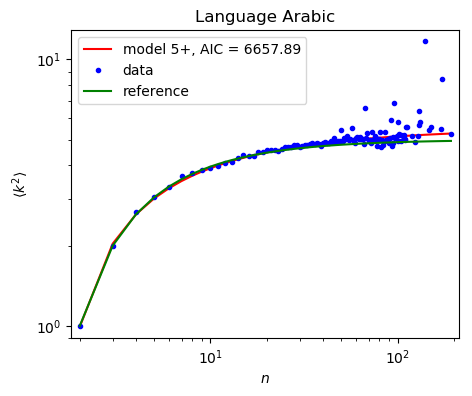
\includegraphics[width=.5\textwidth]{fig/Arabic-mean.png}
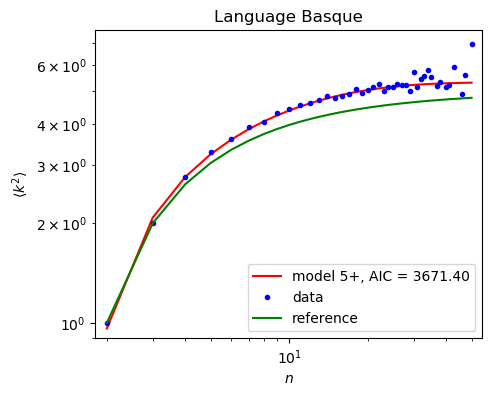
\includegraphics[width=.5\textwidth]{fig/Basque-mean.png}
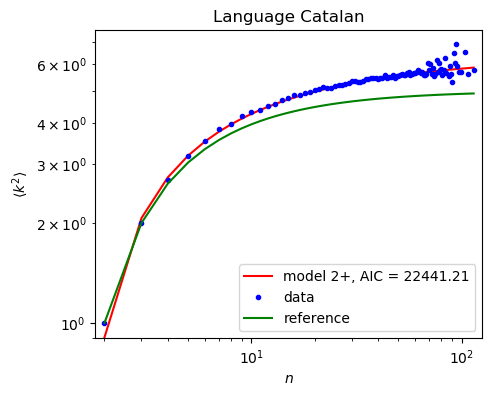
\includegraphics[width=.5\textwidth]{fig/Catalan-mean.png}
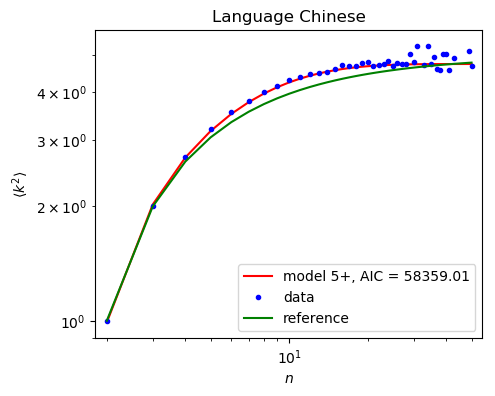
\includegraphics[width=.5\textwidth]{fig/Chinese-mean.png}
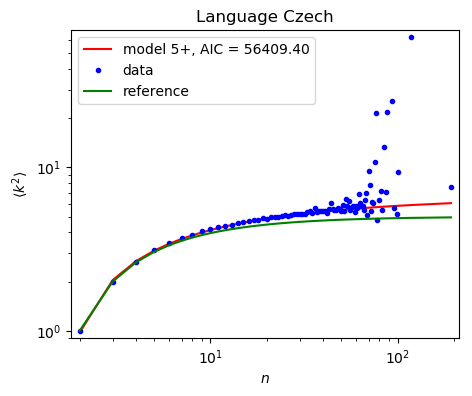
\includegraphics[width=.5\textwidth]{fig/Czech-mean.png}
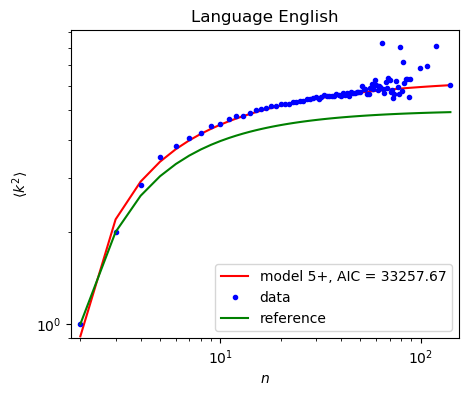
\includegraphics[width=.5\textwidth]{fig/English-mean.png}
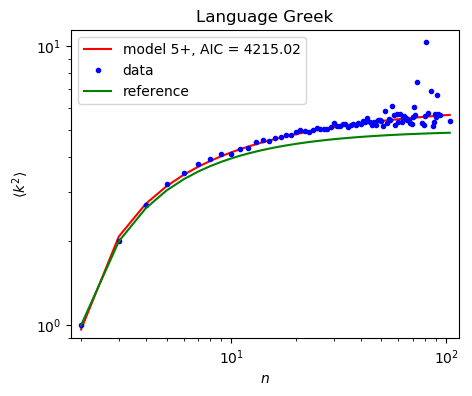
\includegraphics[width=.5\textwidth]{fig/Greek-mean.png}
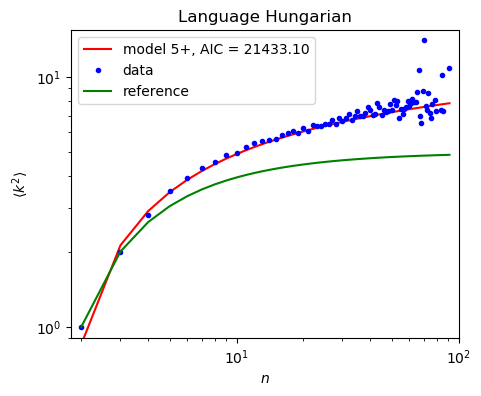
\includegraphics[width=.5\textwidth]{fig/Hungarian-mean.png}
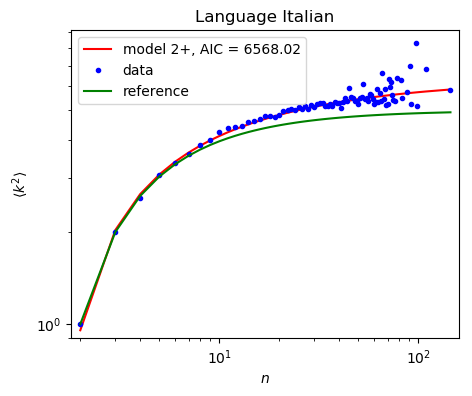
\includegraphics[width=.5\textwidth]{fig/Italian-mean.png}
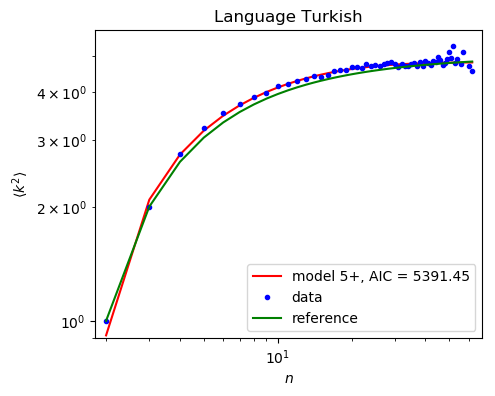
\includegraphics[width=.5\textwidth]{fig/Turkish-mean.png}
%\end{center}


\subsection{Model parameters}
TBD: Fix second table of parameters.
%
\begin{table}[h]
	\centering
	\begin{tabular}{rrrrrrrrrrr}
\toprule
    &   Language &   1 b &   2 a &   2 b &    3 a &    3 c &   4 a &     5 a &    5 b &    5 c \\
\midrule
  1 &      \num{0.405} & \num{0.831} & \num{2.272} & \num{0.001} & \num{11.845} & \num{-0.653} & \num{3.384} & \num{-10.612} & \num{-2.611} &  \num{9.271} \\
  2 &      \num{1.240} & \num{2.148} & \num{3.563} & \num{0.000} & \num{10.588} & \num{-0.543} & \num{3.384} & \num{-10.612} & \num{-3.702} & \num{10.814} \\
  3 &      \num{1.804} & \num{2.936} & \num{4.492} & \num{0.001} &  \num{9.669} & \num{-0.464} & \num{3.384} & \num{-10.612} & \num{-3.854} & \num{10.718} \\
\bottomrule
\end{tabular}
	\caption{The models parameters.}
	\label{tab:params1}
\end{table}
%
%
\begin{table}[h]
	\centering
	\begin{tabular}{lrrrrrrrr}
\toprule
 Language   &   1+ b &   1+ d &    2+ a &   2+ b &   2+ d &   3+ a &   3+ c &   3+ d \\
\midrule
 Arabic     &  \num{0.394} &  \num{1.609} &  \num{-7.046} & \num{-0.647} &  \num{5.493} & \num{-5.193} & \num{-0.179} &  \num{4.839} \\
 Basque     &  \num{0.550} &  \num{1.656} &  \num{-8.393} & \num{-0.616} &  \num{6.386} &  \num{5.000} &  \num{5.000} &  \num{5.000} \\
 Catalan    &  \num{0.372} &  \num{2.456} &  \num{-8.227} & \num{-0.591} &  \num{6.367} & \num{-4.571} & \num{-0.130} &  \num{5.434} \\
 Chinese    &  \num{0.737} &  \num{0.952} &  \num{-8.086} & \num{-0.572} &  \num{6.383} &  \num{5.000} &  \num{5.000} &  \num{5.000} \\
 Czech      &  \num{0.483} &  \num{1.666} &  \num{-7.956} & \num{-0.525} &  \num{6.506} & \num{-5.389} & \num{-0.169} &  \num{5.191} \\
 English    &  \num{0.372} &  \num{2.685} &  \num{-8.594} & \num{-0.664} &  \num{6.342} & \num{-4.741} & \num{-0.147} &  \num{5.536} \\
 Greek      &  \num{0.409} &  \num{2.042} &  \num{-7.831} & \num{-0.594} &  \num{6.157} & \num{-5.291} & \num{-0.162} &  \num{5.210} \\
 Hungarian  &  \num{0.510} &  \num{2.581} & \num{-11.970} & \num{-0.346} & \num{10.312} & \num{-5.949} & \num{-0.083} &  \num{7.418} \\
 Italian    &  \num{0.442} &  \num{1.832} &  \num{-7.905} & \num{-0.546} &  \num{6.370} & \num{-5.462} & \num{-0.170} &  \num{5.187} \\
 Turkish    &  \num{0.463} &  \num{1.680} &  \num{-7.846} & \num{-0.831} &  \num{5.251} &  \num{5.000} &  \num{5.000} &  \num{5.000} \\
\bottomrule
\end{tabular}
	\caption{The models parameters.}
	\label{tab:params2}
\end{table}
%


\section{Results}

\section{Discussion}

\section{Methods}

%\bibliographystyle{unsrt}
%\bibliography{biblio}

\end{document}
